% !TEX root = ../thesis.tex

\chapter{Methodology} \label{chp:methodology}

This chapter elaborates in detail the theoretical framework, technical architecture, and evaluation scheme proposed by this research to address the three core research questions (RQs). The structure of this chapter directly corresponds to the three major research questions: Section 1 introduces the ``Three-Tier Digital Twin Decision Framework'' constructed to answer RQ1, providing a standardized experimental environment for this research; Section 2 deeply analyzes the designed architecture to answer RQ2, elucidating how it addresses the challenges of the physical world; Section 3 defines the evaluation framework and quantitative metrics needed to answer RQ3, particularly the concept of ``Cognitive Gain.''

\section{Three-Tier Digital Twin Framework}

To systematically evaluate the decision-making capabilities of a Large Language Model (LLM) Agent in the physical world and answer the core research question RQ1 (``How can we construct a decision environment framework that reflects the evolutionary complexity of physical decision-making tasks?''), it is essential to first establish a standardized ``capability testing ground.'' Traditional Digital Twin maturity models (such as NASA or ISO 23247 standards) exhibit fundamental inadequacies for this objective \cite{glaessgen2012digital, ISO23247}. These models focus primarily on evaluating the fidelity, integration level, and data coverage of twins from an engineering perspective, but they fail to provide measurement standards for assessing the cognitive challenges that such environments pose to external AI agents.

To address this gap, this research proposes and constructs the \textbf{Three-Tier Digital Twin Decision Framework}. This framework represents a fundamental shift in perspective: it no longer evaluates what twins ``are,'' but rather what types of decisions twins ``can support AI agents to make.'' Based on the progressive escalation of cognitive capability requirements for decision-making tasks, it divides Digital Twin environments into three logically advancing tiers: Descriptive (L1), Predictive (L2), and Interactive (L3). An engineering-wise highly mature twin, if it only contains historical data without predictive models, would still belong to L1 in our framework. This framework provides clear target ladders for the design of the proposed architecture and establishes a consistent and reproducible experimental environment foundation for all subsequent empirical research.

\subsection{Framework Structure and Definitions}

The Three-Tier Digital Twin Decision Framework is structured as follows:

\begin{table}[h]
\centering
\caption{Three-Tier Digital Twin Framework Detailed Specification}
\label{tab:three_tier_framework}
\begin{tabular}{|p{1.5cm}|p{2.5cm}|p{2.5cm}|p{2cm}|p{2cm}|p{2cm}|p{2cm}|}
\hline
\textbf{Tier} & \textbf{Name} & \textbf{Core Function} & \textbf{Decision Type} & \textbf{Data Characteristics} & \textbf{Key Challenges} & \textbf{Case Study} \\
\hline
L1 & Descriptive Twin & Authoritative Record of Reality & Diagnostic (What is?) & Static/quasi-static, structured, multimodal & Information fusion, noise processing & Building Diagnosis \\
\hline
L2 & Predictive Twin & Causal Simulator of Time & Strategic (What if?) & Model-based, requires input, outputs predictions & Model orchestration, parameter understanding & Cancer Treatment Planning \\
\hline
L3 & Interactive Twin & Counterfactual Sandbox for Action & Actionable (What to do?) & Real-time interaction, closed-loop, with delays and consequences & Safety, efficiency, real-time performance & UAV Exploration \\
\hline
\end{tabular}
\end{table}

\subsection{L1 - Descriptive Twin: Authoritative Record of Reality}

The L1 tier represents a high-fidelity ``digital archive'' of the physical world. It integrates multi-source heterogeneous data from physical entities at specific time points or historical periods, including but not limited to geometric and topological information from BIM/CAD models, structured data from relational databases, historical time-series data generated by Internet of Things (IoT) sensors, and unstructured technical documents and inspection reports \cite{tao2018digital, negri2017review}.

At this tier, the core cognitive challenge for agents is diagnosis and attribution. Agents must be able to understand natural language queries about ``current state'' or ``past events'' and accurately transform them into complex, joint queries across different data sources. For example, in the ``building diagnosis'' case study, agents need to integrate structural information from BIM models, dynamic readings from multiple stress sensors, and textual inspection records from engineers to comprehensively assess risk in a specific area \cite{boje2020towards}.

The key challenges of L1 environments lie in information fusion and noise processing, directly testing the data grounding and robustness of the perception module. The complexity arises from the need to handle:
\begin{itemize}
\item \textbf{Heterogeneous Data Integration}: Combining structured databases, time-series sensor data, and unstructured text documents while maintaining semantic coherence \cite{lu2020digital}.
\item \textbf{Temporal Alignment}: Synchronizing data from different sources with varying sampling rates and timestamps.
\item \textbf{Quality Assessment}: Identifying and handling inconsistent, missing, or corrupted data across multiple sources.
\item \textbf{Semantic Mapping}: Translating natural language queries into appropriate database queries, API calls, and file operations.
\end{itemize}

\subsection{L2 - Predictive Twin: Causal Simulator of Time}

The L2 tier builds upon L1 by integrating engineering simulation models with predictive capabilities, constituting the ``causal law engine'' of the physical world. These models (such as Finite Element Analysis, Computational Fluid Dynamics, pharmacokinetic models, etc.) can deduce future system states or responses to interventions based on given input parameters \cite{rasheed2020digital, fuller2020digital}. This enables decisions to leap from ``What happened?'' to ``What will happen if...?''

At this tier, the core cognitive challenge for agents is planning and strategy generation. Agents must engage in forward-looking ``what-if'' reasoning by understanding, selecting, parameterizing, and orchestrating these complex simulation models to evaluate the potential consequences of different strategies. For example, in the ``cancer treatment planning'' case study, agents need to invoke tumor microenvironment simulation models, input different treatment protocols, and compare predicted tumor growth curves to find optimal solutions \cite{rasheed2020digital}.

The key challenges of L2 environments lie in complex model orchestration and semantic understanding of inputs/outputs, directly testing the planning and tool utilization capabilities of the reasoning module. The complexity includes:
\begin{itemize}
\item \textbf{Model Selection}: Choosing appropriate simulation models from available options based on the specific prediction requirements.
\item \textbf{Parameter Configuration}: Understanding complex input requirements and generating appropriate configuration files for simulations.
\item \textbf{Execution Management}: Coordinating potentially long-running simulations while maintaining system responsiveness.
\item \textbf{Result Interpretation}: Extracting meaningful insights from complex simulation outputs, often requiring domain expertise.
\end{itemize}

\subsection{L3 - Interactive Twin: Counterfactual Sandbox for Action}

The L3 tier represents the pinnacle of cognitive challenges, adding closed-loop control interfaces with physical entities or their high-fidelity simulators on top of L2. This means agent decisions are no longer unidirectional analysis or prediction but are transformed into physical actions that can influence environment states in real-time and bidirectionally. The environment responds to agent actions by producing new states and providing feedback, forming a complete ``perception-decision-action'' loop \cite{thrun2002probabilistic}.

At this tier, the core cognitive challenge for agents is safe autonomous action. Agents must not only plan ``what to do'' but also solve the problem of ``how to do it safely and efficiently.'' For example, in the ``UAV exploration'' case study, each movement command from the agent changes the UAV's position and must be executed in real-time within a dynamically changing environment while maintaining safety as the highest priority \cite{grande2012scan}.

The key challenges of L3 environments lie in the trade-offs and assurance among safety, task efficiency, and real-time performance, directly testing the effectiveness of the dual-loop safety execution mechanism of the action module. The complexity encompasses:
\begin{itemize}
\item \textbf{Real-time Constraints}: Making decisions within strict time limits while maintaining safety and effectiveness.
\item \textbf{Safety Assurance}: Ensuring all actions remain within safe operational boundaries despite uncertainties.
\item \textbf{Adaptive Planning}: Modifying plans based on real-time feedback and changing environmental conditions.
\item \textbf{Multi-objective Optimization}: Balancing competing objectives such as task completion, safety, and resource efficiency.
\end{itemize}

\subsection{Framework Validation and Application}

By establishing this cognition-challenge-oriented three-tier framework, this research provides a clear methodology for answering RQ1. It creates a ``testing track'' with progressively increasing cognitive complexity, enabling the core capabilities of the proposed architecture to be independently and systematically evaluated at their corresponding tiers, thereby laying a solid foundation for the overall empirical research of this thesis.

The framework's effectiveness is demonstrated through its ability to:
\begin{itemize}
\item Provide standardized evaluation environments across different complexity levels
\item Enable systematic comparison of different architectural approaches
\item Support incremental capability development and testing
\item Facilitate reproducible research through well-defined experimental conditions
\end{itemize}

\section{CORTEX Architecture Design}

To systematically answer core research question RQ2 (``How can we design an agent architecture that bridges the 'cognitive-physical gap'?''), this section deeply analyzes the technical core of the proposed architecture. The architecture represents not an incremental improvement over existing agent paradigms but a fundamentally redesigned, modular cognitive system for physical world interaction. Its design philosophy positions the LLM as a powerful ``cognitive core'' while consciously recognizing and addressing its inherent deficiencies in physical perception, complex model interaction, and safe execution through dedicated engineering modules.

As illustrated in Figure~\ref{fig:architecture_overview}, the architecture consists of an integrated system containing three highly specialized but tightly coordinated modules: the Perception Module (Grounded Perception), the Reasoning Module (Predictive Reasoning), and the Action Module (Safe Embodied Action). The design of these three modules forms direct, one-to-one correspondence with the three core challenges defined in Section~\ref{chp:intro}—Reality Grounding, Model Utilization, and Safe Execution.

\begin{figure}[htbp]
\centering
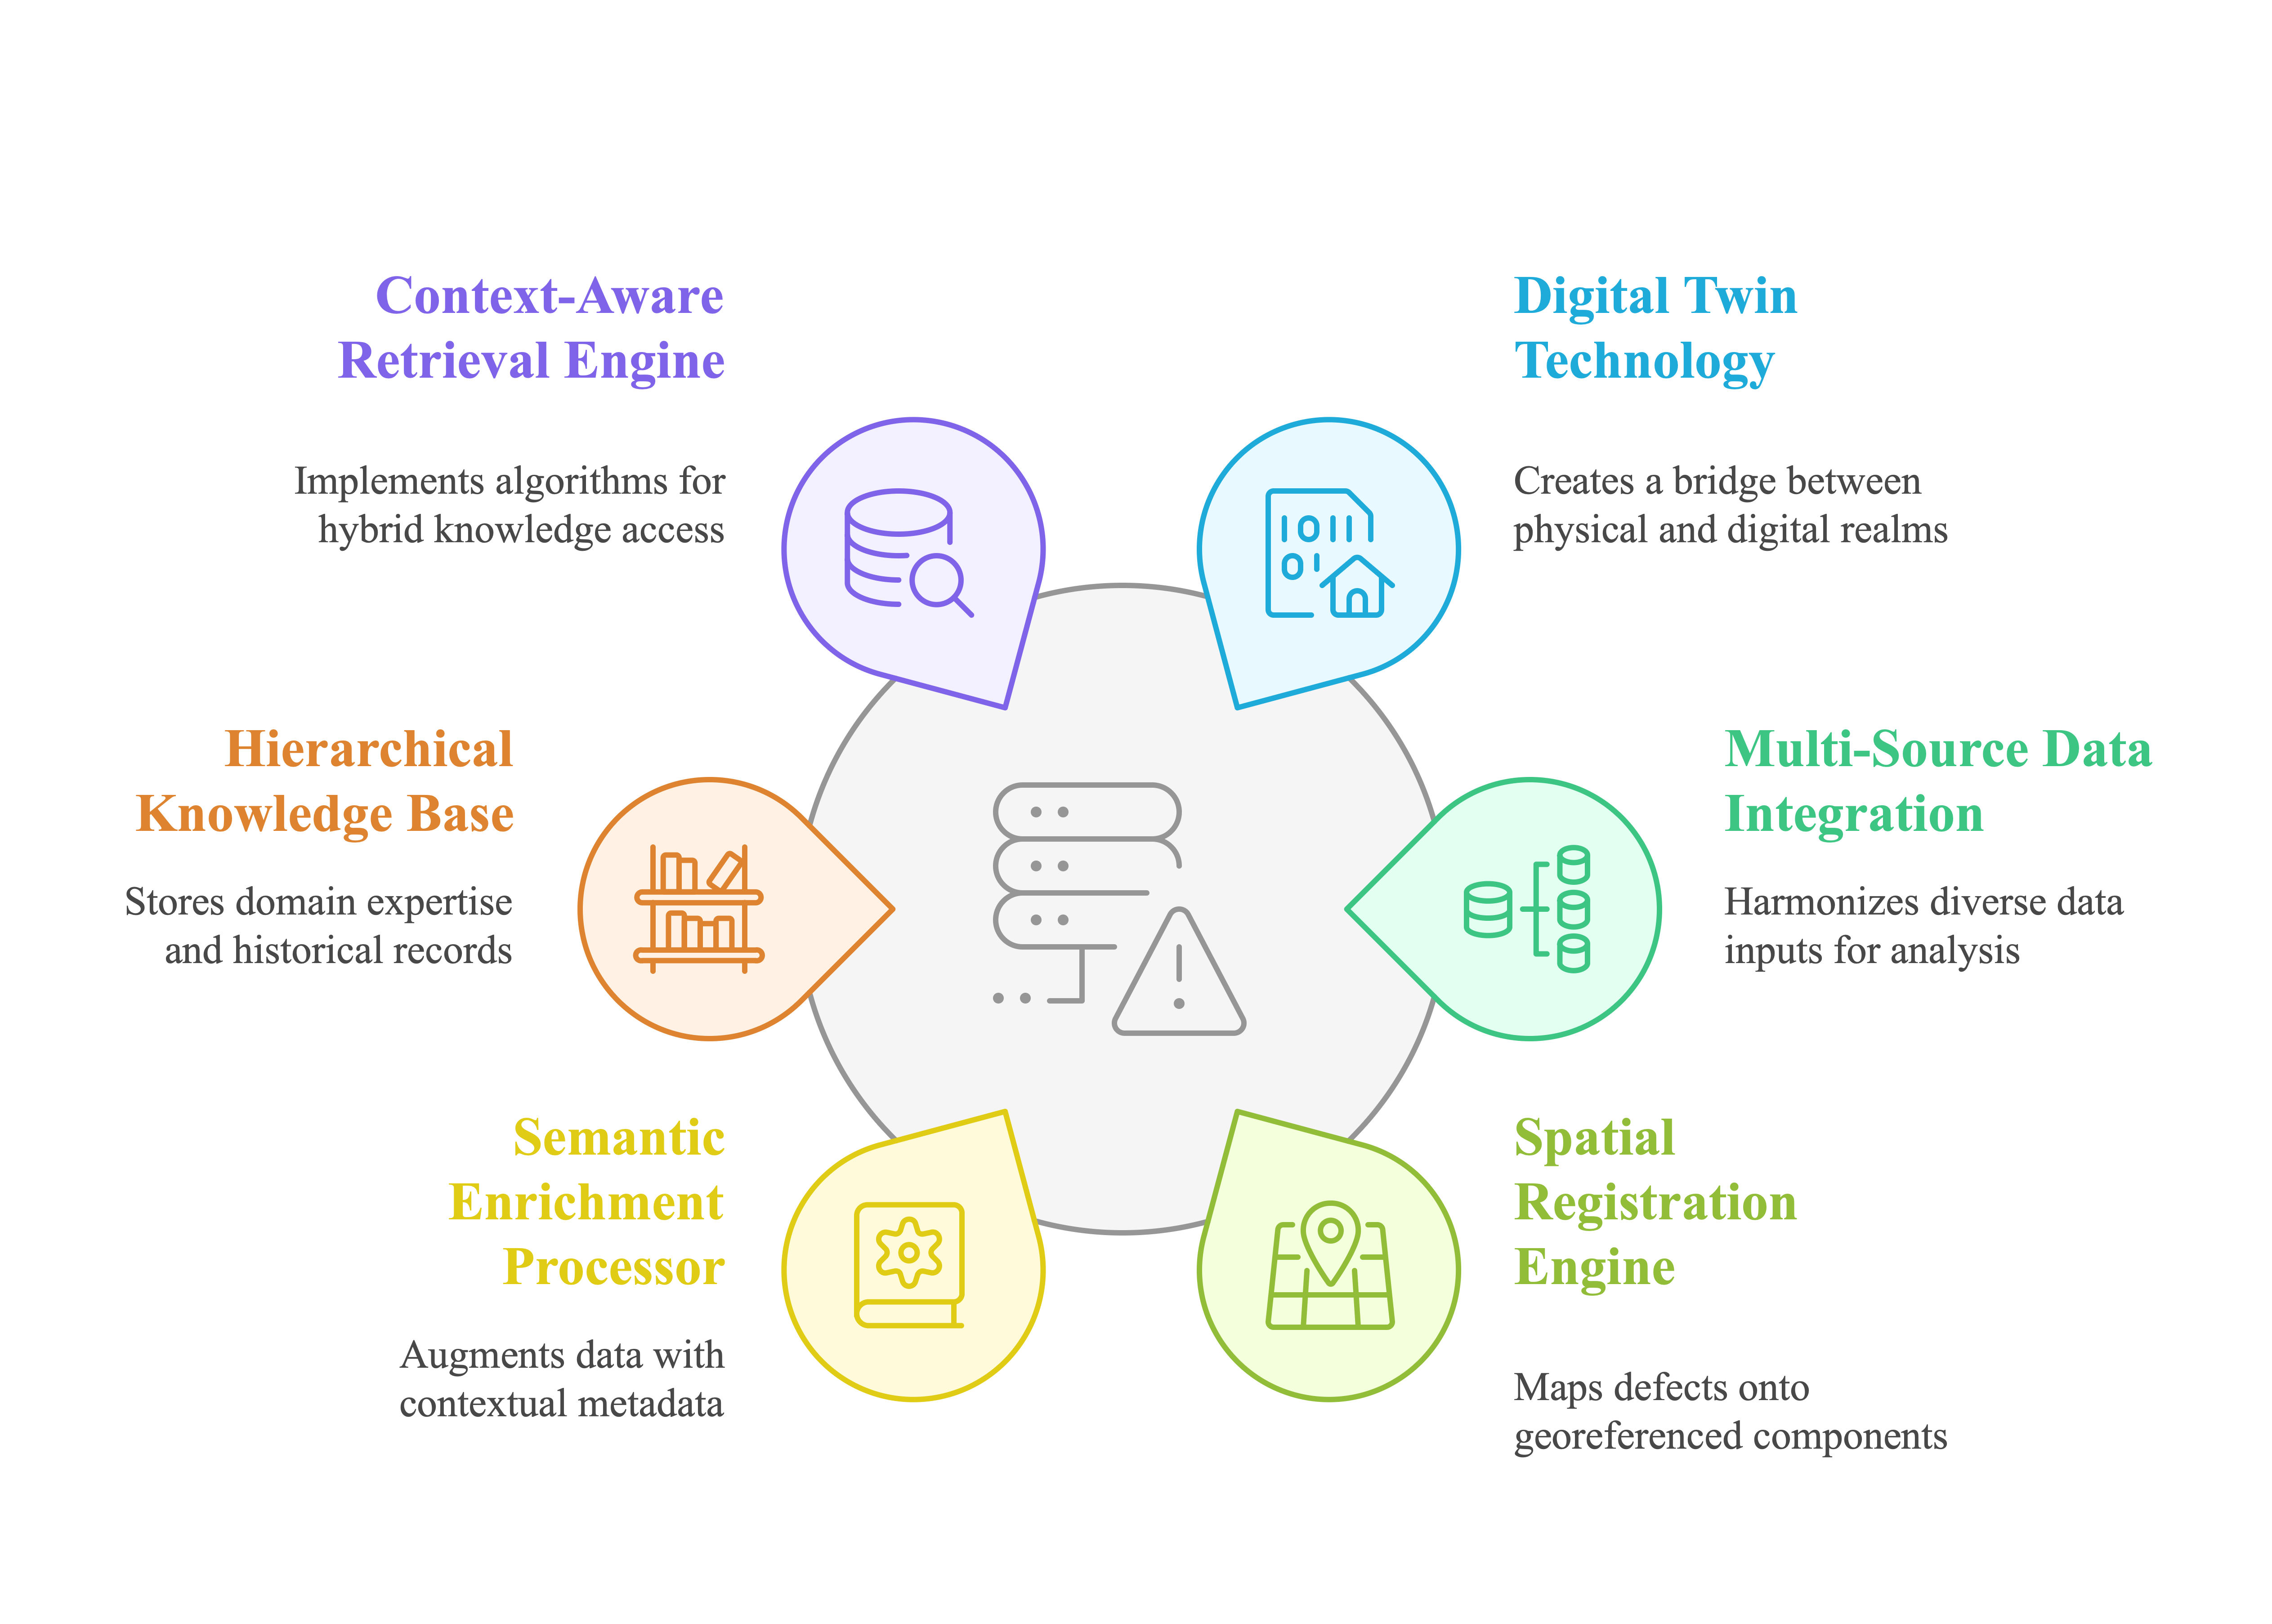
\includegraphics[width=0.9\textwidth]{figures/DefectGPT/Overall Framework.png}
\caption{Architecture Overview: The integrated system showing the three main modules (Perception, Reasoning, Action) and their interfaces with the three-tier Digital Twin environment.}
\label{fig:architecture_overview}
\end{figure}

\subsection{Perception Module: Digital Twin-native Retrieval-Augmented Generation (DT-RAG)}

To address the reality grounding challenge, the Perception Module implements a system called DT-RAG (Digital Twin-native Retrieval-Augmented Generation), achieving deep understanding of physical world data. The primary obstacle to reality grounding stems from the fundamental mismatch between standard RAG paradigms and Digital Twin data characteristics \cite{lewis2020retrieval}.

Digital Twin information environments are structured (such as SQL databases), multimodal (such as BIM geometric models and time-series data), and dynamic, making simple vectorized text retrieval methods completely ineffective. To overcome this obstacle, the Perception Module upgrades the core concept of RAG from ``single retrieval'' to ``intelligent query routing and multimodal knowledge fusion'' \cite{gao2023retrieval}.

\subsubsection{Multi-Modal Data Adapter Suite}

The process begins with a natural language information requirement generated by the Reasoning Module. The DT-RAG intent analyzer first parses this requirement and decomposes it into multiple sub-tasks. Subsequently, these sub-tasks are distributed to a parallel suite of specialized data adapters for execution:

\begin{itemize}
\item \textbf{Structured Data Adapter}: Converts intentions into SQL statements to query asset databases, handling complex joins and aggregations across multiple tables \cite{scholak2021duorat}.
\item \textbf{Time-Series Adapter}: Generates specialized queries to extract sensor readings from time-series databases, including temporal filtering and statistical aggregations \cite{yue2022ts2vec}.
\item \textbf{Document Retrieval Adapter}: Utilizes traditional vector retrieval to search for relevant text within unstructured documents, employing semantic similarity matching \cite{karpukhin2020dense}.
\item \textbf{Geometric Model Adapter}: Makes specialized API calls to extract spatial and geometric information from BIM models, including spatial queries and geometric calculations \cite{boje2020towards}.
\end{itemize}

\subsubsection{Information Fusion and Contextualization}

The heterogeneous results returned by these parallel queries require sophisticated fusion mechanisms. The most critical step in DT-RAG is integrating these information fragments into a unified, context-rich textual summary. This fusion process involves:

\begin{itemize}
\item \textbf{Semantic Alignment}: Ensuring that information from different sources refers to the same physical entities or phenomena.
\item \textbf{Temporal Synchronization}: Aligning data from different time periods and sampling rates into coherent temporal narratives.
\item \textbf{Quality Weighting}: Assigning confidence scores to different information sources based on reliability and relevance.
\item \textbf{Contextual Summarization}: Generating natural language summaries that preserve essential quantitative relationships while being optimized for LLM comprehension.
\end{itemize}

This summary is ultimately injected into the LLM's prompt, transforming a raw and unreadable physical environment into preprocessed, grounded knowledge that the LLM can directly understand and reason about, fundamentally resolving the LLM's ``hallucination'' problem in physical domains \cite{ji2023survey}.

\subsection{Reasoning Module: Model-Profile-Driven Deep Tool Orchestration}

Building upon the resolved data grounding issue, the Reasoning Module focuses on addressing the more advanced ``model utilization'' challenge. Physical world decision-making often requires leveraging complex engineering simulation models (such as FEA, CFD) for forward-looking prediction, yet these models are semantically opaque ``black boxes'' for existing LLM agents \cite{hughes2012finite}.

The architecture addresses this challenge through a ``model-profile-driven deep tool orchestration'' mechanism, elevating the LLM's role from a simple API caller to a ``virtual systems engineer'' \cite{lu2022unified}.

\subsubsection{Model Profile System}

In this architecture, every complex physical model is encapsulated as a ``tool'' and equipped with a detailed ``Model Profile.'' This profile is a semi-structured description that details:

\begin{itemize}
\item \textbf{Functional Specification}: What the model simulates and under what conditions it is applicable.
\item \textbf{Input Requirements}: Complex input formats including configuration files, boundary conditions, and parameter specifications.
\item \textbf{Execution Protocol}: Precise command sequences, expected runtime, and resource requirements.
\item \textbf{Output Structure}: Format and interpretation of simulation results, including visualization options.
\item \textbf{Domain Guidelines}: Expert knowledge for interpreting results and understanding limitations.
\end{itemize}

\subsubsection{Multi-Step Engineering Orchestration}

When facing an L2-level task requiring prediction, the LLM's reasoning chain becomes a multi-step orchestration process following rigorous engineering logic rather than single-step tool invocation:

\begin{enumerate}
\item \textbf{Task Analysis}: Understanding the prediction requirements and identifying appropriate simulation models.
\item \textbf{Configuration Generation}: Dynamically generating compliant input configuration files based on task objectives and model profiles.
\item \textbf{Execution Management}: Invoking execution commands for potentially long-running simulations while monitoring progress.
\item \textbf{Result Processing}: Analyzing output results using model profile interpretation guidelines and calling data analysis tools.
\item \textbf{Insight Generation}: Forming high-level insights based on physical model evidence and domain knowledge.
\end{enumerate}

This deep interaction capability enables the architecture to truly harness professional engineering knowledge within Digital Twins, systematically solving the challenge of combining LLMs with complex physical models \cite{lu2022unified}.

\subsection{Action Module: Slow-Fast Dual-Loop Coordination Mechanism}

When decisions need to be translated into physical actions, the Action Module addresses the most critical ``safe execution'' challenge. Directly applying slow, non-deterministic LLM reasoning to systems requiring high-frequency, deterministic, and safety-first physical operations creates irreconcilable contradictions \cite{amodei2016concrete}.

To resolve this risk, the Action Module innovatively designs a ``Slow-Fast Dual-Loop Coordination Mechanism,'' completely decoupling decision-making ``thinking'' from ``execution.'' This mechanism draws inspiration from and modernizes classical deliberative-reactive control theory in robotics \cite{gat1998three}.

\subsubsection{Dual-Loop Architecture}

The mechanism consists of two interconnected but independent control loops:

\textbf{Slow Loop (Cognitive Brain)}: 
\begin{itemize}
\item Driven by the LLM serving as the system's cognitive ``brain''
\item Responsible for deliberate, globally-informed macro-strategic planning
\item Operates at lower frequency to fully leverage LLM's cognitive intelligence
\item Generates high-level commands and strategic objectives
\item Monitors long-term performance and adjusts strategies accordingly
\end{itemize}

\textbf{Fast Loop (Deterministic Spinal Cord)}:
\begin{itemize}
\item Independent of the LLM, implemented as a real-time process in high-performance languages
\item Continuously monitors low-level sensors at extremely high frequency
\item Receives macro-commands from the slow loop
\item Possesses absolute safety review authority over all instructions
\item Executes immediate emergency responses when safety violations are detected
\end{itemize}

\subsubsection{Safety-First Execution Protocol}

The core innovation lies in the fast loop's absolute safety review authority. Before executing any action, it performs comprehensive safety verification:

\begin{enumerate}
\item \textbf{Constraint Verification}: Ensuring all actions satisfy predefined safety boundaries (maximum torque, minimum safety distance, etc.).
\item \textbf{Real-time Monitoring}: Continuously checking environmental conditions and system states.
\item \textbf{Emergency Override}: Immediately interrupting tasks and executing predefined safety procedures when risks are detected.
\item \textbf{Feedback Generation}: Providing error feedback to the slow loop for strategy adjustment.
\end{enumerate}

This clear responsibility separation elegantly resolves the conflict between advanced cognition and physical safety, providing a solid and reliable architectural foundation for deploying LLM agents in dynamic, unpredictable physical worlds, thus providing a complete answer to RQ2.

\section{Evaluation Framework and Metrics}

To systematically answer core research question RQ3 (``How can we quantitatively validate the effectiveness of the proposed architecture through rigorous evaluation?''), this section provides detailed specifications for experimental design and performance metrics. The evaluation framework aims to objectively measure the advantages of the proposed approach over traditional methods through carefully designed controlled experiments and comprehensive metric systems, particularly the core concept of \textbf{``Cognitive Gain''} representing performance improvement \cite{stone2016artificial}.

\subsection{Experimental Design and Methodology}

The evaluation employs a rigorous controlled comparison scheme to highlight the cognitive capability benefits brought by the proposed architecture. Specifically, for each case study (corresponding to the L1, L2, L3 tier tasks described above), two types of experimental subjects are established for comparison: one category consists of intelligent agents enabled with the proposed architecture + LLM (experimental group), and the other category consists of optimized traditional best methods in the respective domains (control group) \cite{duan2022survey}.

\subsubsection{Controlled Experiment Design}

This comparison can be viewed as a type of ``ablation experiment'': by maintaining completely identical environmental and task conditions while introducing the proposed architecture's cognitive modules as the only variable, we can ensure that any observed performance differences primarily stem from the advanced cognitive capabilities within the architecture \cite{rogers2021primer}.

The experimental design philosophy emphasizes fairness and reproducibility:

\begin{itemize}
\item \textbf{Environmental Parity}: Both experimental and control groups access identical Digital Twin data, simulation models, and task specifications.
\item \textbf{Task Equivalence}: All groups receive identical objective functions, constraints, and success criteria.
\item \textbf{Resource Constraints}: Computational resources and time limits are standardized across all experimental conditions.
\item \textbf{Statistical Rigor}: Multiple trials with proper randomization and statistical significance testing.
\end{itemize}

For example, in the L1 building diagnosis task, both groups access the same Digital Twin data; in the L2 medical decision task, both groups base their protocol development on identical patient information and simulation models; in the L3 UAV exploration task, both systems execute equivalent task objectives in identical simulated environments.

\subsubsection{Baseline Selection and Validation}

The selection of appropriate baselines is crucial for meaningful evaluation. For each tier, baselines are chosen based on:

\begin{itemize}
\item \textbf{State-of-the-art Performance}: Current best-performing methods in each domain
\item \textbf{Practical Deployment}: Methods that have been successfully deployed in real-world scenarios
\item \textbf{Algorithmic Diversity}: Representative approaches from different methodological families
\item \textbf{Fair Comparison}: Methods that operate under similar computational and information constraints
\end{itemize}

\subsection{Key Performance Indicators (KPIs)}

To comprehensively characterize performance, the evaluation employs multi-dimensional core performance indicators covering three major aspects: task effectiveness, decision quality, and robustness with adaptability \cite{hernandez2022measuring}.

\subsubsection{Task Effectiveness Metrics}

Task effectiveness indicators directly reflect the agent's ability to complete tasks quantitatively or qualitatively:

\begin{itemize}
\item \textbf{Success Rate}: Percentage of tasks completed successfully within specified constraints
\item \textbf{Coverage Rate}: Proportion of problem space explored or addressed (e.g., area covered in UAV exploration)
\item \textbf{Completion Time}: Time required to achieve task objectives
\item \textbf{Resource Utilization}: Computational, energy, or material resources consumed during task execution
\item \textbf{Throughput}: Number of tasks completed per unit time in batch processing scenarios
\end{itemize}

\subsubsection{Decision Quality Metrics}

Decision quality indicators measure the optimality and appropriateness of agent-generated decisions or solutions:

\begin{itemize}
\item \textbf{Expert Agreement}: Consistency between agent recommendations and expert judgments, measured through inter-rater reliability metrics
\item \textbf{Optimality Gap}: Difference between agent solutions and theoretical or empirically-determined optimal solutions
\item \textbf{Risk Assessment Accuracy}: Precision and recall in identifying potential hazards or failure modes
\item \textbf{Consistency}: Stability of decisions across similar scenarios or repeated trials
\item \textbf{Interpretability}: Clarity and logical coherence of decision explanations and justifications
\end{itemize}

For example, in medical protocol planning, this manifests as consistency scores between proposed treatment protocols and recommendations from oncology expert panels; in building diagnosis, it appears as accuracy in structural risk assessment (precisely identifying actual hidden dangers while avoiding false positives) \cite{rasheed2020digital}.

\subsubsection{Robustness and Adaptability Metrics}

Robustness and adaptability indicators evaluate the agent's ability to maintain performance under non-ideal conditions:

\begin{itemize}
\item \textbf{Noise Tolerance}: Performance degradation curves when sensor data contains varying levels of noise
\item \textbf{Environmental Adaptation}: Ability to maintain effectiveness under changing environmental conditions
\item \textbf{Failure Recovery}: Speed and effectiveness of recovery from component failures or unexpected events
\item \textbf{Generalization}: Performance maintenance when deployed in scenarios different from training conditions
\item \textbf{Learning Efficiency}: Rate of performance improvement over time with accumulated experience
\end{itemize}

For instance, testing building diagnosis accuracy degradation curves when sensor data contains certain noise levels, or introducing sudden obstacles in UAV exploration tasks to observe system replanning efficiency and safety \cite{grande2012scan}.

\subsection{Cognitive Gain: A Comprehensive Performance Metric}

To intuitively quantify the overall advantages achieved by the proposed architecture relative to traditional baseline approaches, we introduce \textbf{``Cognitive Gain''} as a comprehensive indicator. Cognitive Gain aims to express the performance improvement magnitude brought by advanced cognitive capabilities in percentage form \cite{stone2016artificial}.

\subsubsection{Mathematical Definition}

For metrics where higher values indicate better performance, Cognitive Gain is defined as:

\begin{equation}
\text{Cognitive Gain (\%)} = \left(\frac{\text{Metric}_{\text{Proposed}}}{\text{Metric}_{\text{Baseline}}} - 1\right) \times 100\%
\end{equation}

For example, if the proposed intelligent agent achieves a 90\% success rate in a task while the traditional baseline method achieves 75\%, the Cognitive Gain for success rate would be approximately 20\%.

For metrics where lower values indicate better performance (such as error rates or completion times), we use equivalent processing through reciprocals or difference measures to ensure consistent interpretation of Cognitive Gain.

\subsubsection{Multi-Dimensional Cognitive Gain Analysis}

Cognitive Gain is not merely focused on single metric improvement but aims to capture the total advantage gained through introducing cognitive intelligence. In actual analysis, we calculate Cognitive Gain for each case study's key indicators separately and discuss them in combination with qualitative results, evaluating the practical value of the proposed architecture from multiple perspectives \cite{hernandez2022measuring}.

The comprehensive analysis includes:

\begin{itemize}
\item \textbf{Primary Metrics}: Core performance indicators most relevant to each application domain
\item \textbf{Secondary Metrics}: Supporting indicators that provide additional insights into system behavior
\item \textbf{Interaction Effects}: How improvements in one metric may influence others
\item \textbf{Domain Specificity}: Which types of cognitive gains are most pronounced in different application areas
\item \textbf{Scalability}: How cognitive gains change with problem complexity or scale
\end{itemize}

\subsubsection{Statistical Significance and Confidence Intervals}

To ensure robust and reliable conclusions, Cognitive Gain measurements include:

\begin{itemize}
\item \textbf{Statistical Testing}: Appropriate hypothesis tests to determine significance of observed gains
\item \textbf{Confidence Intervals}: Uncertainty bounds around Cognitive Gain estimates
\item \textbf{Effect Size}: Practical significance of observed differences beyond statistical significance
\item \textbf{Power Analysis}: Ensuring sufficient sample sizes for reliable detection of meaningful differences
\end{itemize}

\subsection{Evaluation Protocol and Procedures}

The evaluation follows a standardized protocol ensuring consistent and reproducible results across all case studies:

\subsubsection{Pre-Evaluation Phase}

\begin{enumerate}
\item \textbf{Environment Setup}: Standardized configuration of Digital Twin environments and baseline systems
\item \textbf{Calibration}: Verification that all systems operate within expected parameters
\item \textbf{Baseline Validation}: Confirmation that baseline methods achieve expected performance levels
\item \textbf{Metric Specification}: Clear definition of all evaluation metrics and measurement procedures
\end{enumerate}

\subsubsection{Evaluation Execution}

\begin{enumerate}
\item \textbf{Randomization}: Proper randomization of test scenarios and initial conditions
\item \textbf{Parallel Testing}: Simultaneous evaluation of experimental and control conditions where possible
\item \textbf{Data Collection}: Systematic recording of all relevant performance metrics and system behaviors
\item \textbf{Quality Assurance}: Real-time monitoring for evaluation integrity and data quality
\end{enumerate}

\subsubsection{Post-Evaluation Analysis}

\begin{enumerate}
\item \textbf{Statistical Analysis}: Comprehensive statistical testing of collected data
\item \textbf{Cognitive Gain Calculation}: Computation of Cognitive Gain metrics with appropriate uncertainty quantification
\item \textbf{Qualitative Analysis}: Interpretation of quantitative results with domain expert insights
\item \textbf{Validation}: Cross-validation of results and sensitivity analysis for key findings
\end{enumerate}

\subsection{Chapter Summary}

Through the establishment of the above evaluation framework, this research lays a solid foundation for answering RQ3. Rigorous controlled experimental design ensures fair and effective comparisons, multi-dimensional indicator systems guarantee comprehensive and in-depth evaluation, and ``Cognitive Gain'' as a refined indicator provides intuitive means for quantifying the value of advanced cognitive architectures.

The framework enables systematic assessment of the proposed architecture's capabilities across the three-tier Digital Twin environment while providing quantitative evidence for the benefits of integrating LLM reasoning with physical world interaction. The next chapters will report and analyze the experimental processes and results of three case studies under this framework, providing empirical validation of the theoretical contributions presented in this methodology chapter.

The evaluation methodology ensures that conclusions about the architecture's effectiveness are based on rigorous empirical evidence rather than anecdotal observations, supporting the broader goal of advancing the field of intelligent physical world interaction through principled research and development.